\documentclass[twoside,11pt]{article}

\usepackage[T1]{fontenc}
\usepackage{amsmath}
\usepackage{booktabs}
\usepackage{microtype}
\usepackage{xcolor}
\usepackage{caption}
\usepackage{subcaption}
\usepackage{enumitem}
\usepackage{url}
\usepackage{jmlr2e}
\usepackage{lastpage}

\setlength{\tabcolsep}{3pt}
\captionsetup{font=small,labelfont=bf}

\jmlrheading{}{2026}{1-\pageref{LastPage}}{11/26}{}{}{Varadaraj Acharya}
\ShortHeadings{Neurons or Subspaces?}{Acharya}
\firstpageno{1}

\title{Neurons or Subspaces?\\[2pt]
Calibration-Sensitive Refusal in Open Instruction Models}

\author{\name Varadaraj Acharya \email{varadaraj277@gmail.com} \\
        \addr Independent Researcher\\
        Udupi, Karnataka, India}

\editor{Action Editor}

\begin{document}
\maketitle

\begin{abstract}
Safety-aligned language models refuse harmful requests, but the mechanism is
contested: is refusal implemented by a sparse set of MLP neurons, or by a linear
direction in the residual stream? We study this question on four open instruction
models using minimally paired harmful/benign prompts from JailbreakBench, a brutal
HarmBench transfer set, and a content-matched style control. Ablating a
mean-difference direction removes refusal in Qwen3.5-0.8B (53.3\% $\to$ 0.0\%) and
DeepSeek-R1-Distill-1.5B (26.7\% $\to$ 6.7\%), and transfers to HarmBench
(42.0\% $\to$ 0.0\% and 31.1\% $\to$ 6.7\%). LFM3-1.7B is calibration-sensitive:
the matched direction reduces refusal only from 86.7\% to 73.3\%, while a direction
estimated on a larger natural corpus reaches 82.0\% $\to$ 21.0\% at a KL cost of
1.05. Qwen3.5-4B is the strongest refusal model and the hardest case:
96.7\% $\to$ 50.0\% at KL 1.16, with HarmBench 93.3\% $\to$ 42.0\%. Removing the
direction at a single layer is much weaker than removing it at every layer, so the
effect is distributed rather than localised. Neuron clamping is
model-dependent: 80 neurons across four layers reduce refusal to 20.0\% in
Qwen3.5-0.8B, leave R1-Distill unchanged at 26.7\%, reduce LFM3 to 36.7\%, and
leave Qwen3.5-4B at 96.7\%. Adding the direction induces refusal but at a large
distribution cost (KL up to 4.45). We conclude that refusal is a distributed,
calibration-sensitive linear mechanism---not a single neuron, and not a universal
layer or direction.
\end{abstract}

\begin{keywords}
refusal, mechanistic interpretability, activation steering, calibration, safety alignment
\end{keywords}

\section{Introduction}

Instruction-tuned language models are trained to refuse harmful requests while
remaining helpful on benign ones. The safety behaviour is remarkably consistent
across model families, yet its internal implementation is still debated. One view
holds that refusal is a \emph{sparse circuit}: a small set of MLP neurons that fire
on harmful intent and route generation into a refusal template. The other holds
that refusal is a \emph{linear direction} in the residual stream, spread across
layers, which can be projected out or added at inference time.

The linear view has strong recent support. \citet{arditi2024refusal} identify a
single difference-in-means direction in thirteen chat models and show that erasing
it prevents refusal while adding it induces refusal on harmless instructions. This
is a striking result, but three questions remain open.

First, \emph{is the direction an artefact of prompt style?} The standard evaluation
contrasts AdvBench harmful requests with Alpaca instructions. The two sets differ in
topic, length, and mood: harmful prompts are usually imperatives (``Write a
ransomware script''), while benign prompts are often questions (``How do I change a
tire?''). A mean-difference direction can therefore encode request style as much as
harmfulness.

Second, \emph{is the direction universal?} A direction estimated on one corpus may
not transfer to another, and the literature rarely reports how sensitive the
estimate is to the calibration distribution.

Third, \emph{do neurons matter?} Single-neuron ablation studies often test fewer
than 1\% of the MLP at a single, often final, layer. That is a narrow test of a
broad hypothesis.

We address these questions with a controlled study on four heterogeneous open
models: a hybrid linear-attention VLM (Qwen3.5-0.8B), a reasoning-distilled Qwen2
model (DeepSeek-R1-Distill-1.5B), a hybrid short-conv/attention model
(LFM3-1.7B), and a higher-refusal hybrid VLM (Qwen3.5-4B). Our evaluation uses:
(i) \emph{minimally paired} JailbreakBench prompts, where each harmful request has a
benign counterpart with the same template, topic and length;
(ii) a \emph{brutal external} HarmBench set, never seen during calibration;
(iii) a \emph{style control} that renders the same benign prompts as imperatives and
as questions; and
(iv) a \emph{neuron budget} sweep from 1 to 5\% of the MLP, including multi-layer
clamping.

\paragraph{Contributions.}
\begin{enumerate}[leftmargin=1.4em,itemsep=2pt,topsep=2pt]
\item A matched-pair evaluation of refusal directions that removes the
imperative-vs-question and topic confounds of AdvBench-vs-Alpaca designs, with a
content-matched style direction as a negative control.
\item Evidence that the refusal direction is \emph{calibration-sensitive}: it is
strong in Qwen3.5-0.8B and R1-Distill, but in LFM3-1.7B the matched direction is
weak while a natural-corpus direction is strong, at a higher KL cost.
\item A brutal transfer test: a direction estimated on moderate JBB pairs ablates
refusal on HarmBench for three of four models.
\item A neuron-budget study showing that single-layer top-$k$ clamping is weak
everywhere, while 80 neurons across four layers can substantially reduce refusal in
some models and not others.
\item A fully reproducible pipeline, including disjoint splits, random-direction
and random-neuron controls, Wilson intervals, and KL cost.
\end{enumerate}

\section{Related Work}

\paragraph{Refusal directions and activation steering.}
\citet{arditi2024refusal} compute a difference-in-means direction at the last
instruction token and show that directional ablation bypasses refusal across
thirteen models. Activation addition \citep{turner2023activation} and contrastive
activation addition \citep{panickssery2023steering} use comparable interventions for
style and sentiment. Our ablation follows the same all-layer scope; our contribution
is the matched-pair evaluation, the calibration analysis, and the neuron comparison.

\paragraph{Geometry of refusal.}
\citet{marshall2024affine} show that refusal is better described by an affine
function than by a pure direction, and that directional ablation alone can produce
incoherent outputs. \citet{wollschlager2025cones} identify multiple independent
refusal directions and multi-dimensional concept cones. Our results are consistent
with a dominant direction but not with exclusivity: the estimate is
calibration-sensitive and the intervention has a measurable distribution cost.

\paragraph{Neuron-level safety.}
\citet{chen2024safetyneurons} identify a small fraction of safety neurons and show
that patching them restores much of the safety behaviour. This is compatible with
our finding that single neurons are insufficient but multi-layer neuron clamping can
matter; the two literatures differ in budget, layer choice, and causal score.

\paragraph{Reliability of steering.}
\citet{tan2024reliability} show that steering vectors can be unreliable across
prompts and can have opposite-of-intended effects. We therefore report held-out
prompt-level rates, random controls, and KL rather than a single prompt.

\paragraph{Evaluation benchmarks.}
JailbreakBench \citep{chao2024jailbreakbench} provides paired harmful and benign
behaviours with matching categories. HarmBench \citep{mazeika2024harmbench} provides
a large, more severe behaviour set. AdvBench \citep{zou2023universal} is the common
harmful corpus; Alpaca is the common benign one. Our design uses JBB for the matched
test and HarmBench for external severity, and reserves AdvBench/Alpaca for layer
selection.

\section{Method}

\subsection{Refusal direction}

For each layer $l$, let $\mu_l^{+}$ and $\mu_l^{-}$ be the mean residual-stream
activations at the last prompt token for harmful and benign calibration prompts.
The refusal direction is
\begin{equation}
r_l = \frac{\mu_l^{+} - \mu_l^{-}}{\lVert \mu_l^{+} - \mu_l^{-}\rVert_2}.
\end{equation}
The decision token is the final token of the chat-formatted prompt. For Qwen3.5 and
LFM3 we disable thinking so that the first generated token is the answer; for
R1-Distill we prefill an empty \texttt{</think>} block for the same reason.

\subsection{Layer selection}

The layer is chosen on an independent natural validation split (96 harmful / 48
harmless AdvBench/Alpaca prompts), not on the matched test distribution. For each
candidate layer we compute (i) the mean refusal score on harmful validation prompts
after all-layer ablation, (ii) the mean refusal score on harmless prompts after
adding the direction, and (iii) the KL divergence on harmless prompts. We prune the
last 20\% of layers and choose
\begin{equation}
L^{\star} = \arg\min_{l \,:\, \mathrm{KL}_l \le 0.1} s^{\mathrm{abl}}_l .
\end{equation}
This follows the selection logic of \citet{arditi2024refusal} and avoids the
``largest separation norm'' heuristic, which is biased toward the final layer.

\subsection{Interventions}

\paragraph{Ablation.} We project the unit direction out of the embedding output and
every block output:
\begin{equation}
h \leftarrow h - (h^{\top} r)\, r .
\end{equation}
The \emph{single-layer} control applies the same projection only at $L^{\star}$.

\paragraph{Addition.} We add the direction at $L^{\star}$ to all token positions,
\begin{equation}
h \leftarrow h + \alpha r, \qquad \alpha = m\,\lVert \mu^{+}_{L^{\star}} - \mu^{-}_{L^{\star}}\rVert_2 ,
\end{equation}
with $m \in \{0, 0.5, 1, 1.5, 2\}$. This matches the scale used by
\citet{arditi2024refusal}.

\subsection{Neuron attribution and clamping}

For layer $L^{\star}$ and intermediate neuron $j$, we score
\begin{equation}
S_j = \bigl(\mathbb{E}^{+}[a_j] - \mathbb{E}^{-}[a_j]\bigr)\,
      \bigl(r_{L^{\star}}^{\top} W_{\mathrm{down}}[:,j]\bigr),
\end{equation}
where $a_j$ is the pre-down-projection MLP activation. We clamp the top-$k$ neurons
to zero at every token position. We test $k \in \{1, 5, 20, 100, 500, 5\%\}$ of the
MLP and compare against three random neuron sets. The multi-layer variant splits a
budget across $\{L^{\star}-2, \ldots, L^{\star}+1\}$, scoring each layer with the
same direction and clamping the top neurons per layer.

\subsection{Metrics}

The refusal score at the last prompt token is
\begin{equation}
s = \log p(\mathcal{R}) - \log\bigl(1 - p(\mathcal{R})\bigr),
\end{equation}
where $\mathcal{R}$ is the set of refusal-initiating first tokens (\texttt{I},
\texttt{As}, \texttt{Sorry}, \texttt{No}) and $p(\mathcal{R})$ is their total
probability mass. A prompt counts as a refusal when $s > 0$ (equivalently,
$p(\mathcal{R}) > 0.5$). We report Wilson 95\% intervals. KL is the mean divergence
of the next-token distribution on harmless prompts versus the unmodified model.

\subsection{Controls}

\paragraph{Random direction.} A random unit vector of the same norm is ablated and
added, averaged over three draws.

\paragraph{Random neurons.} Three random neuron sets of the same cardinality are
clamped and averaged.

\paragraph{Style direction.} The same benign JBB prompts are rendered as imperatives
and as questions (content matched). The difference-in-means direction is a pure
mood axis; we report its cosine with the refusal direction and the effect of
ablating it.

\paragraph{External brutal set.} A direction estimated on JBB is evaluated unchanged
on HarmBench standard behaviours; the benign side is JBB benign prompts from the
mapped domain.

\section{Experimental Setup}

\paragraph{Models.} Table~\ref{tab:setup} lists the models. Qwen3.5 is a hybrid
linear/full-attention VLM; we use its text stack. LFM3 is a hybrid short-conv and
attention model loaded with its remote code. R1-Distill is a standard Qwen2
transformer. Qwen3.5-4B is a larger hybrid VLM with a much higher baseline refusal
rate (96.7\% on JBB), which makes it the hardest case in the study.

\begin{table}[t]
\centering
\small
\caption{Models. All four models are evaluated; Qwen3.5-4B is the high-refusal
case.}
\label{tab:setup}
\begin{tabular}{lccccc}
\toprule
Model & Family & Layers & $d$ & $d_{\mathrm{MLP}}$ & Status \\
\midrule
Qwen3.5-0.8B & qwen3\_5 & 24 & 1024 & 3584 & complete \\
R1-Distill-1.5B & qwen2\_r1 & 28 & 1536 & 8960 & complete \\
LFM3-1.7B & lfm3 & 24 & 2048 & 7680 & complete \\
Qwen3.5-4B & qwen3\_5 & 32 & 2560 & 9216 & complete \\
\bottomrule
\end{tabular}
\end{table}

\paragraph{Data.} The direction is estimated on 50 matched JBB pairs; the layer is
chosen on 96/48 AdvBench/Alpaca prompts; the main test is 30 held-out JBB pairs. The
external set is 119 HarmBench standard behaviours, paired with JBB benign prompts
from the same domain. The style control uses 50 benign JBB prompts in imperative and
question form. Calibration, validation and test prompts are disjoint.

\paragraph{Compute.} Apple M5 Pro (24 GB), MPS, float16, PyTorch 2.15.0 and
Transformers 5.22.1. Prompts are batched with left padding; generation is greedy.

\section{Results}

\subsection{Directional ablation}

Table~\ref{tab:main} and Figure~\ref{fig:bars} report the held-out matched-pair
results. All-layer ablation removes refusal in Qwen3.5-0.8B (53.3\% $\to$ 0.0\%)
and R1-Distill (26.7\% $\to$ 6.7\%). LFM3-1.7B is the exception: the matched
direction reduces refusal only from 86.7\% to 73.3\%. Qwen3.5-4B is the strongest
refusal model and the hardest case: 96.7\% $\to$ 50.0\% at KL 1.16, so the
direction is real but the intervention is incomplete. Single-layer ablation is much
weaker in every model (10.0\%, 13.3\%, 70.0\%, 90.0\%), so the mechanism is
distributed across the residual stream rather than localised at $L^{\star}$. A
random unit direction leaves the refusal score essentially unchanged
($\Delta \in [-0.09, +0.13]$), while the estimated direction lowers it
substantially (for example, from $+0.13$ to $-4.05$ in Qwen3.5-0.8B).

\begin{table}[t]
\centering
\small
\caption{Held-out JBB matched-pair results. Rates are percent with 95\% Wilson
intervals. $\Delta$ random is the change in mean refusal log-odds under a random
unit direction (three draws). KL is on JBB benign prompts.}
\label{tab:main}
\resizebox{\linewidth}{!}{\begin{tabular}{lcccccc}
\toprule
Model & Layer & Baseline (\%) & Ablated (\%) & Single-layer (\%) & $\Delta$ random & KL \\
\midrule
Qwen3.5-0.8B & 12 & 53.3 [36.1, 69.8] & 0.0 [0.0, 11.4] & 10.0 [3.5, 25.6] & $+0.10$ & 0.568 \\
R1-Distill-1.5B & 15 & 26.7 [14.2, 44.4] & 6.7 [1.8, 21.3] & 13.3 [5.3, 29.7] & $-0.02$ & 0.367 \\
LFM3-1.7B & 8 & 86.7 [70.3, 94.7] & 73.3 [55.6, 85.8] & 70.0 [52.1, 83.3] & $+0.13$ & 0.193 \\
Qwen3.5-4B & 9 & 96.7 [83.3, 99.4] & 50.0 [33.2, 66.8] & 90.0 [74.4, 96.5] & $-0.09$ & 1.159 \\
\bottomrule
\end{tabular}}
\end{table}

\begin{figure}[t]
\centering
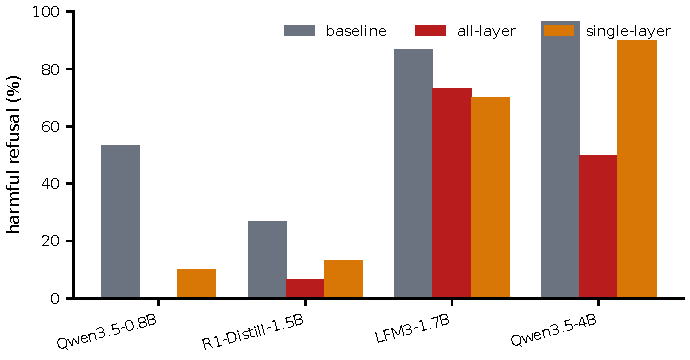
\includegraphics[width=0.82\linewidth]{figures/main_bars.pdf}
\caption{Harmful refusal before and after direction ablation, and under the
single-layer control. The all-layer intervention is the causal effect; the
single-layer bar shows that removing the direction at one layer is not enough.}
\label{fig:bars}
\end{figure}

\subsection{Layer selection and calibration sensitivity}

Figure~\ref{fig:sweep} shows the validation ablation score by layer. The selected
layers are 12 (Qwen3.5-0.8B), 15 (R1-Distill), 8 (LFM3-1.7B) and 9
(Qwen3.5-4B); the curves are smooth and the selected layer is not the last block.
The choice is model-specific and does not collapse to a single depth.

Table~\ref{tab:calibration} re-estimates the direction on the 96-prompt natural
corpus and tests it on all 100 JBB pairs. Qwen3.5-0.8B and R1-Distill are stable
(51.0\% $\to$ 0.0\% and 28.0\% $\to$ 7.0\%). Qwen3.5-4B is also stable but
incomplete (93.0\% $\to$ 40.0\%, KL 1.70). LFM3-1.7B changes from a weak
matched-direction effect (86.7\% $\to$ 73.3\%) to a strong natural-direction effect
(82.0\% $\to$ 21.0\%), at KL 1.05 versus 0.19. The refusal direction in LFM3 is
therefore real but its \emph{estimate} depends on the calibration distribution.

\begin{figure}[t]
\centering
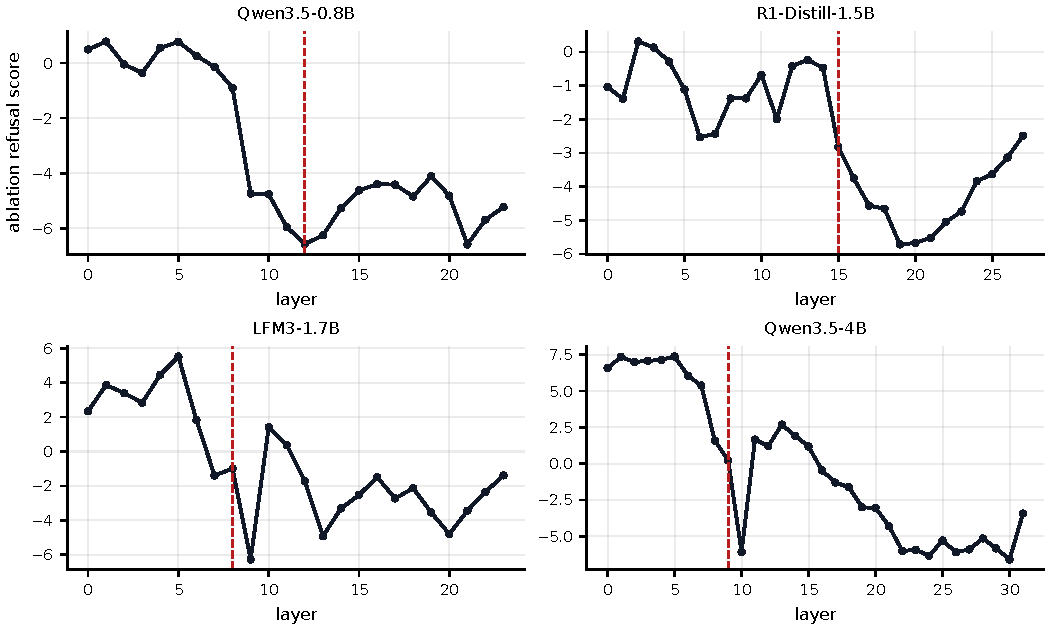
\includegraphics[width=\linewidth]{figures/layer_sweep.pdf}
\caption{Validation ablation refusal score by layer. The dashed line marks the
selected layer. Lower is better.}
\label{fig:sweep}
\end{figure}

\begin{table}[t]
\centering
\small
\caption{Calibration sensitivity: direction re-estimated on 96 natural prompts and
tested on all 100 JBB pairs. HarmBench is the brutal external set.}
\label{tab:calibration}
\resizebox{\linewidth}{!}{\begin{tabular}{lccccc}
\toprule
Model & Layer & Baseline (\%) & Ablated (\%) & KL & HarmBench (\%) \\
\midrule
Qwen3.5-0.8B & 12 & 51.0 & 0.0 & 0.978 & 42.0 $\to$ 0.0 \\
R1-Distill-1.5B & 15 & 28.0 & 7.0 & 0.204 & 31.1 $\to$ 13.5 \\
LFM3-1.7B & 8 & 82.0 & 21.0 & 1.048 & 65.5 $\to$ 23.5 \\
Qwen3.5-4B & 9 & 93.0 & 40.0 & 1.700 & 93.3 $\to$ 34.4 \\
\bottomrule
\end{tabular}}
\end{table}

\subsection{Brutal transfer}

Table~\ref{tab:external} evaluates the JBB direction on 119 HarmBench standard
behaviours. Refusal drops from 42.0\% to 0.0\% in Qwen3.5-0.8B and from 31.1\% to
6.7\% in R1-Distill, with small KL on the benign side (0.28). Qwen3.5-4B drops from
93.3\% to 42.0\%. LFM3-1.7B does not transfer (65.5\% $\to$ 63.0\%), consistent
with its calibration sensitivity. The matched direction therefore generalises to
much more severe prompts in three of four models, but not universally.

\begin{table}[t]
\centering
\small
\caption{HarmBench transfer. The direction is computed on JBB pairs; the benign
side is JBB benign prompts from the mapped domain.}
\label{tab:external}
\resizebox{\linewidth}{!}{\begin{tabular}{lccccc}
\toprule
Model & Brutal baseline (\%) & Brutal ablated (\%) & Benign baseline (\%) & Benign ablated (\%) & KL \\
\midrule
Qwen3.5-0.8B & 42.0 & 0.0 & 1.7 & 0.0 & 0.284 \\
R1-Distill-1.5B & 31.1 & 6.7 & 10.9 & 1.7 & 0.280 \\
LFM3-1.7B & 65.5 & 63.0 & 11.8 & 7.6 & 0.160 \\
Qwen3.5-4B & 93.3 & 42.0 & 19.3 & 2.5 & 0.753 \\
\bottomrule
\end{tabular}}
\end{table}

\subsection{Style control}

Table~\ref{tab:style} reports the imperative-vs-question direction. It is nearly
orthogonal to the refusal direction in Qwen3.5-0.8B ($\cos=-0.16$), R1-Distill
($\cos=-0.03$) and Qwen3.5-4B ($\cos=-0.21$), and ablating it does not reproduce
the effect: Qwen3.5-0.8B falls only to 23.3\%, while R1-Distill and LFM3-1.7B move
to 93.3\% and Qwen3.5-4B to 100.0\% (refusal \emph{increases}). The main direction
is therefore not the mood axis.

\begin{table}[t]
\centering
\small
\caption{Style control: the same benign prompts as imperatives and as questions.
$\cos$ is with the refusal direction at $L^{\star}$.}
\label{tab:style}
\resizebox{\linewidth}{!}{\begin{tabular}{lcccc}
\toprule
Model & $\cos$ & Baseline (\%) & Style-ablated (\%) & KL \\
\midrule
Qwen3.5-0.8B & $-0.156$ & 53.3 & 23.3 & 0.388 \\
R1-Distill-1.5B & $-0.030$ & 26.7 & 93.3 & 2.615 \\
LFM3-1.7B & $-0.093$ & 86.7 & 93.3 & 0.355 \\
Qwen3.5-4B & $-0.210$ & 96.7 & 100.0 & 0.731 \\
\bottomrule
\end{tabular}}
\end{table}

\subsection{Neuron ablation}

Table~\ref{tab:neurons} and Figure~\ref{fig:neurons} show that single-layer neuron
clamping is weak: at 5\% of the MLP, refusal is 40.0\% in Qwen3.5-0.8B (from a
53.3\% baseline), 26.7\% in R1-Distill (unchanged), 93.3\% in LFM3-1.7B (from
86.7\%), and 96.7\% in Qwen3.5-4B (unchanged). The multi-layer budget is more
effective: 80 neurons across four layers reduce refusal to 20.0\% in Qwen3.5-0.8B
(KL 0.13) and 36.7\% in LFM3-1.7B (KL 0.77), but leave R1-Distill at 26.7\% and
Qwen3.5-4B at 96.7\%; the 4B model needs 1840 neurons to reach 80.0\% (KL 0.93).
Random neuron sets do not match the top-$k$ effect in Qwen3.5-0.8B or LFM3-1.7B.
Neurons are neither irrelevant nor a universal switch; their causal role depends on
the model and on the layer budget.

\begin{table}[t]
\centering
\small
\setlength{\tabcolsep}{2.5pt}
\caption{Neuron ablation at about 5\% of the MLP, and 80 neurons across four layers.
Random score is the mean refusal log-odds under three random sets.}
\label{tab:neurons}
\resizebox{\linewidth}{!}{\begin{tabular}{lccccccc}
\toprule
Model & $k$ & \% MLP & Top-$k$ rate (\%) & Top-$k$ score & Random score & Multi-80 rate (\%) & Multi-80 KL \\
\midrule
Qwen3.5-0.8B & 179 & 4.99 & 40.0 & -0.36 & +0.05 & 20.0 & 0.13 \\
R1-Distill-1.5B & 448 & 5.00 & 26.7 & -1.01 & -0.78 & 26.7 & 0.08 \\
LFM3-1.7B & 384 & 5.00 & 93.3 & +2.06 & +1.93 & 36.7 & 0.77 \\
Qwen3.5-4B & 460 & 4.99 & 96.7 & +5.02 & +5.64 & 96.7 & 0.46 \\
\bottomrule
\end{tabular}}
\end{table}

\begin{figure}[t]
\centering
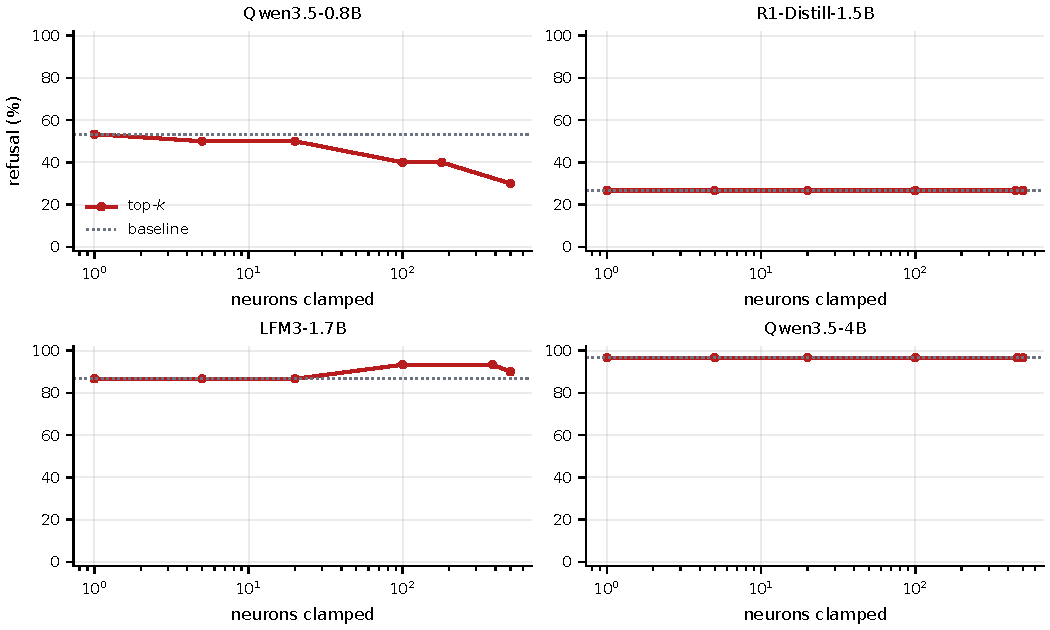
\includegraphics[width=\linewidth]{figures/neurons.pdf}
\caption{Refusal rate versus the number of clamped neurons at $L^{\star}$. The
dotted line is the unmodified baseline. Single-layer clamping is weak; the
multi-layer budget in Table~\ref{tab:neurons} is the stronger intervention.}
\label{fig:neurons}
\end{figure}

\subsection{Addition}

Table~\ref{tab:addition} and Figure~\ref{fig:dose} report the dose-response on
harmless JBB prompts. At $1\times$ the direction raises refusal to 26.7\% in
Qwen3.5-0.8B (KL 0.84), 23.3\% in R1-Distill (KL 0.23), 73.3\% in LFM3-1.7B
(KL 1.90), and 73.3\% in Qwen3.5-4B (KL 1.43). At $2\times$ the rates are 66.7\%,
53.3\%, 63.3\% and 100.0\%, with KL 2.91, 0.93, 3.49 and 4.45. The direction is a
real bidirectional knob, but it is not free: the KL cost is substantial, and
LFM3-1.7B is non-monotonic. A high refusal rate is not by itself evidence of a
clean intervention.

\begin{table}[t]
\centering
\small
\caption{Adding the direction to harmless JBB prompts. KL is versus the unmodified
model.}
\label{tab:addition}
\resizebox{\linewidth}{!}{\begin{tabular}{lcccc}
\toprule
Model & 1.0$\times$ refusal (\%) & 1.0$\times$ KL & 2.0$\times$ refusal (\%) & 2.0$\times$ KL \\
\midrule
Qwen3.5-0.8B & 26.7 & 0.84 & 66.7 & 2.91 \\
R1-Distill-1.5B & 23.3 & 0.23 & 53.3 & 0.93 \\
LFM3-1.7B & 73.3 & 1.90 & 63.3 & 3.49 \\
Qwen3.5-4B & 73.3 & 1.43 & 100.0 & 4.45 \\
\bottomrule
\end{tabular}}
\end{table}

\begin{figure}[t]
\centering
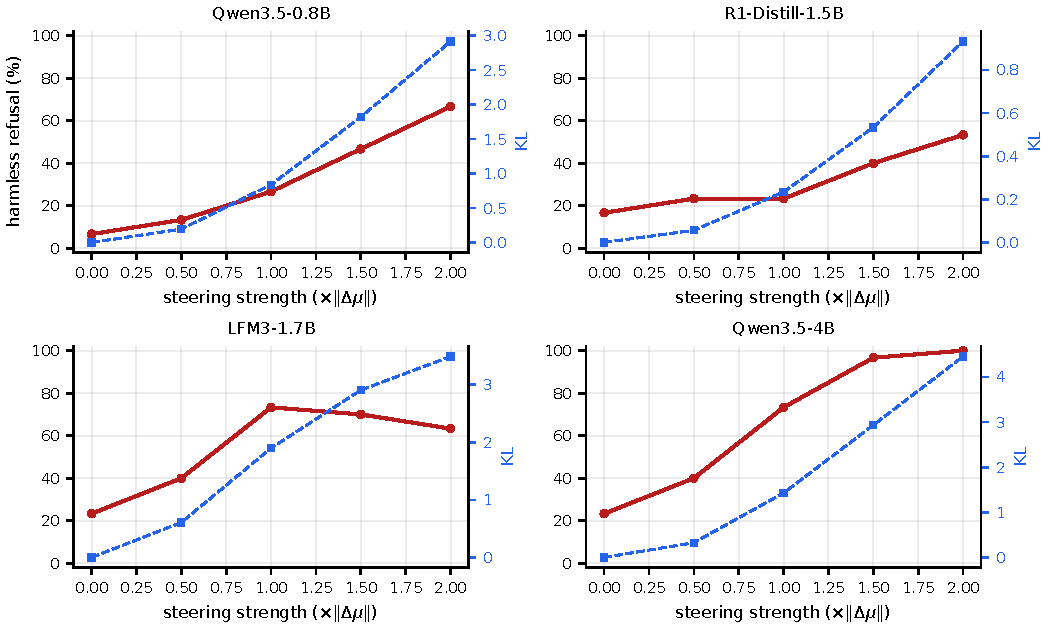
\includegraphics[width=\linewidth]{figures/dose.pdf}
\caption{Refusal on harmless prompts (left axis) and KL versus the unmodified model
(right axis) as the addition strength increases.}
\label{fig:dose}
\end{figure}

\section{Discussion}

\paragraph{A direction, but not a universal one.}
The mean-difference direction is a real causal object: it removes refusal when
projected out, induces it when added, and a random direction does neither. But the
estimate is calibration-sensitive. LFM3-1.7B is the clearest case: the matched
direction barely moves refusal, while a natural-corpus direction moves it strongly
at higher KL. Qwen3.5-4B is a different failure mode: the direction is strong but
incomplete (96.7\% $\to$ 50.0\%) and costly (KL 1.16). The field should report
calibration sensitivity and residual refusal rather than a single direction per
model.

\paragraph{Neurons versus subspaces is not a binary.}
Single neurons are not the mechanism. At 1--20 neurons nothing happens anywhere. At
5\% of the MLP, single-layer clamping is still weak; across four layers it becomes
effective in Qwen3.5-0.8B and LFM3-1.7B, but not in R1-Distill or Qwen3.5-4B. The
right question is not ``neurons or subspaces?'' but ``which distributed subspace,
at which budget, in which architecture?''.

\paragraph{The cost of steering.}
Adding the direction induces refusal, but KL rises to 1--4.5~nats and the response
can degenerate. A safety intervention that damages harmless behaviour is not
deployable, and a jailbreak that produces incoherent text is not a clean jailbreak.
Reporting KL alongside refusal is necessary.

\paragraph{Implications for safety.}
If refusal is a thin linear offset, white-box safety is brittle: a few dozen
calibration prompts and a forward hook can disable it. The brittleness is not
uniform---architecture and calibration matter---but it is real, and it argues for
defences that do not live only in a removable direction.

\section{Limitations}

\begin{itemize}[leftmargin=1.2em,itemsep=2pt,topsep=2pt]
\item Four models and three architecture families. Qwen3.5-4B is the high-refusal
case and its matched direction is incomplete (50\% residual) with KL 1.16; a larger
model may behave differently, and scaling the study is future work.
\item Refusal is a proxy for harmfulness. We report log-odds and a string
classifier, not an LLM judge or StrongREJECT score. A compliant answer can still be
useless or incoherent; a refusal can be a topic restatement.
\item Greedy decoding only; we do not estimate sampling variance.
\item The matched test is 30 pairs. The external HarmBench set is category-matched,
not minimally edited, so it tests severity generalisation rather than the confound.
\item R1-Distill is evaluated with an empty thinking block; its refusal behaviour
under normal chain-of-thought may differ.
\item LFM3-1.7B is calibration-sensitive; the matched direction is weak and the
natural direction has a higher KL. We report both rather than choose the favourable
one.
\end{itemize}

\section{Ethics Statement}

This work studies why models refuse and how that behaviour can be removed. It is
dual-use: the same intervention that audits a safety mechanism can bypass it. We use
public benchmark prompts, do not introduce a new attack, and do not include
operational harmful content in this paper. Qualitative samples were reviewed
locally and are not redistributed. We report the cost of the intervention (KL)
rather than presenting a jailbreak as a free lunch. We encourage responsible
disclosure and the use of these results to build defences that are not a single
removable direction.

\section{Reproducibility}

The repository contains the runner, dataset construction, and table and figure
generators under \texttt{src/}. The repository is available
at \newline \url{https://github.com/varadaraj772/neuron-subspace}. The matched,
external, style and neuron experiments are reproduced by
\begin{verbatim}
python src/study.py --model qwen35_08b
python src/study.py --model lfm3_17b
python src/study.py --model r1distill_15b \
    --model-path models/r1
python src/study.py --model qwen35_4b \
    --model-path models/qwen35_4b \
    --dataset jbb --test-dataset same --force-layer 9
python src/make_tables.py
python src/make_figures.py
\end{verbatim}
All splits are seeded and disjoint; the random controls use fixed seeds. The
calibration-sensitivity runs (Table~\ref{tab:calibration}) are produced by omitting
\texttt{--dataset jbb --test-dataset same --force-layer 9}, which estimates the
direction on the natural split and tests it on all 100 JBB pairs.

\acks{This work was conducted independently, without external funding. The author
declares no competing interests.}

\bibliography{references}

\appendix

\section{Hyperparameters}

\begin{table}[h]
\centering
\small
\begin{tabular}{lcc}
\toprule
Setting & Value & Notes \\
\midrule
Calibration pairs (JBB) & 50 & direction estimate \\
Layer-selection prompts & 96 / 48 & AdvBench / Alpaca \\
Matched test pairs & 30 & held out \\
HarmBench behaviours & 119 & external \\
Style pairs & 50 & imperative vs question \\
Batch size & 8 & left padding \\
Generation & greedy & max 96 tokens \\
Dtype & float16 & MPS \\
Seeds & 0 & splits, controls \\
\bottomrule
\end{tabular}
\caption{Hyperparameters for the main runs.}
\end{table}

\section{Redacted qualitative samples}

We do not reproduce operational harmful text. The repository stores aggregate
metrics, not model completions; qualitative samples were reviewed locally and are
not redistributed. A typical pattern is: the baseline refuses (``I can't assist with
that''); the ablated model complies, and the operational text is omitted here.

\section{Full intervals}

The main table reports 95\% Wilson intervals. The calibration, external, style and
addition tables report point estimates for space; the JSON artifacts contain the
corresponding intervals. The intervals are wide for the 30-pair matched test
(roughly $\pm 15$ percentage points at 50\%) and narrow for the 119-prompt external
set.

\end{document}
